\section{Estado del arte}

Entre los trabajos que se han desarrollado mostrando relación con el proyecto son los siguientes: \\

\begin{enumerate}
	\item SALVEO, es un sistema inteligente de teleasistencia y de monitoreo para personas mayores o discapacitadas que viven solas en casa. El sistema consiste en módulos con sensores de movimiento, los cuales están ubicados en diferentes partes estratégicas de la casa, esto hace que el módulo detecte una eventual caída, o un cambio brutal en el estilo de vida de la persona, a su vez envían la información captada por los sensores a la base de transmisión; de igual manera cuenta con sensores de temperatura los cuales envían esta magnitud a la base de transmisión, lo cual permite controlar la temperatura ambiente y detecta el aumento sospechoso de la temperatura ambiente o eventuales problemas del sistema de calefacción de la casa \cite{treintaycuatro}. 
	
	\begin{figure}[h]
		\centering
		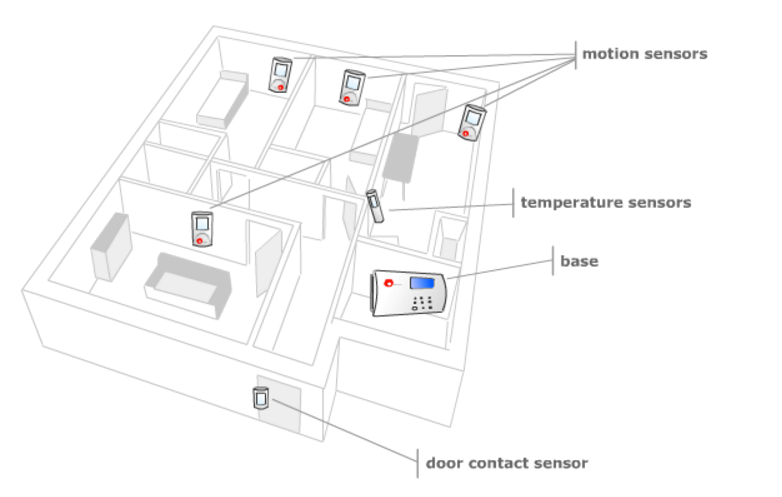
\includegraphics[scale=0.45]{introduccion/imagenes/salveo}
		\textbf{\caption{\small{Representación del sistema SALVEO \cite{treintaycuatro}.}}}
		\label{Seccion1.6:Figura1.18}
	\end{figure}

	\item TESIS IPN, ESIME ZACATENCO, CLASIFICACIÓN: GPI 2012: “Implementación de Sistema de Seguridad con Video-Vigilancia y Software Libre”, el sistema cuenta con cámaras que tienen una configuración para la detección de movimiento y cuando ocurre una eventualidad, envían alarmas por medio de correo electrónico, este sistema utiliza el software libre ZoneMinder \cite{treintaycinco}.
	
	\begin{figure}[h]
		\centering
		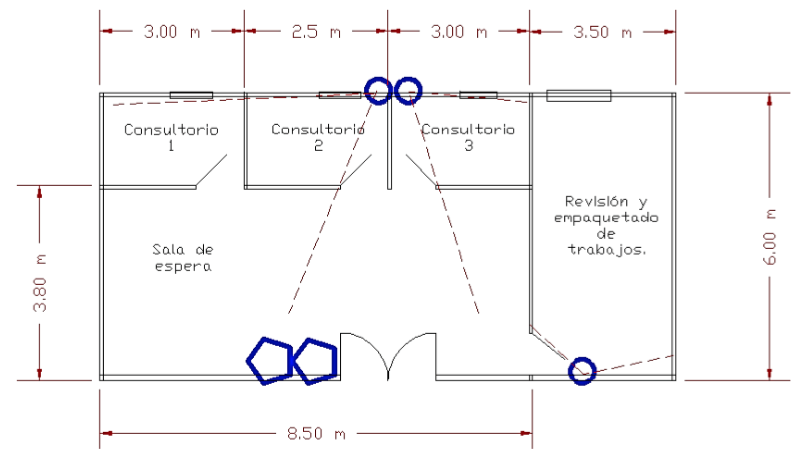
\includegraphics[scale=0.30]{introduccion/imagenes/video_vigilancia}
		\textbf{\caption{\small{Plano de la Implementación de Sistema de Seguridad con Video-Vigilancia y Software Libre  \cite{treintaycinco}.}}}
		\label{Seccion1.6:Figura1.19}
	\end{figure}

	\item Escuela Politécnica del Ejército. ESPE: “Implementación de control de acceso y monitorización para personas con discapacidad mediante un dispositivo móvil”. 
	
	En el siguiente trabajo de tesis muestra la implementación de un control de acceso y monitorización para una persona con discapacidad mediante un dispositivo móvil, el medio de comunicación que ocupa es intranet, con el propósito de ser controlado remotamente dentro de una red, el objetivo del proyecto está enfocado en coadyuvar a personas con discapacidad motriz, facilitando el mando de luces y apertura de compuertas constatando la monitorización con una cámara IP.
	
	\begin{figure}[h]
		\centering
		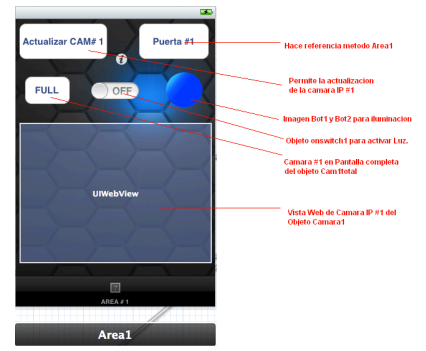
\includegraphics[scale=0.35]{introduccion/imagenes/espe}
		\textbf{\caption{\small{Acción de los objetos al aplicativo \cite{treintayseis}.}}}
		\label{Seccion1.6:Figura1.20}
	\end{figure} 
	
	\item Sense 4 Care, la empresa Sense 4 Care desarrolla dispositivos para monitorear a personas de la tercera edad con el fin de detectar las caídas que puedan sufrir, por medio de un sensor acelerómetro y una aplicación desarrollada en la plataforma Android, con el propósito de mandar un mensaje de alerta a sus familiares y llevar a cabo de forma automática la comunicación, también cuenta con geolocalización no importando si la persona se encuentra en un lugar cerrado o al aire libre \cite{treintaysiete}.
	
	\item Sistema de Red inalámbrica para la vigilancia de la salud: ritmo cardíaco y sensor de temperatura. 
	Este sistema consta del módulo Arduino hardware micro-controlador y software, un sensor de temperatura, un sensor de frecuencia cardíaca, una radio XBee y el protocolo de comunicación inalámbrica. El sensor se envuelve alrededor de la muñeca. Se muestra la frecuencia cardíaca y la temperatura corporal media en un LCD de caracteres, cifra los datos y los transmite a una computadora remota a través de una red XBee. El coordinador está conectado a un PC con un programa para controlar y procesar los datos entrantes \cite{treintayocho}.
	
	\begin{figure}[h]
		\centering
		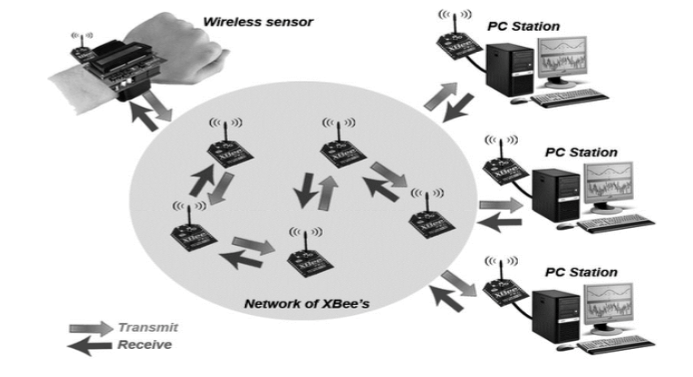
\includegraphics[scale=0.55]{introduccion/imagenes/red_inalambrica}
		\textbf{\caption{\small{Diagrama esquemático del Sistema de Red inalámbrica para la vigilancia de la salud: ritmo cardíaco y sensor de temperatura \cite{treintayocho}.}}}
		\label{Seccion1.6:Figura1.20}
	\end{figure}
	
	\item Smartwatch.
	El fundador de la empresa Cualli Software, creo el primer smartwatch que monitorea remotamente en tiempo real el estado de salud de usuarios adultos mayores, con la finalidad de darle la seguridad que alguien está al pendiente de él las 24 horas, aun sin habitar en la misma casa. Su idea fue diseñar un brazalete que supervise constantemente a un adulto mayor que vive solo y no pueda recibir ayuda en caso de emergencia médica, inspeccionando los signos vitales por medio de tres sensores, uno que mide el pulso otro la temperatura y por último el de movimiento, igualmente incluye un canal de audio unas bocinas pequeñas y un micrófono para que el usuario se comunique a un call center y así se verifiquen sus signos vitales o con los parientes vía Smartphone. Actualmente no ha salido al mercado debido a que están en pruebas \cite{treintaynueve}.
	
	\begin{table}
		\centering
		\begin{tabular}{|p{3cm}|p{6cm}|p{3cm}|}
			\hline
			\centering Software & \centering Características & \centering Precio en el mercado \\
			\tabularnewline
			\hline
			Sistema inteligente de tele asistencia SALVEO &	Permite detectar situaciones anormales, la enfermera o las personas ayudantes pueden tener acceso a la información del estado de la persona mayor, lo que facilita su control. Está compuesto de un sistema inalámbrico de sensores que envían la información percibida a una base de transmisión. & 300\euro \\
			\hline
			Implementación de Sistema de Seguridad con Video-Vigilancia y Software Libre & Se implementó un sistema de seguridad de video-vigilancia, capaz de realizar avisos remotos (por medio de un mensaje de correo electrónico), utilizando cámaras de distintas características y distinto fabricante. & 12,000MXN \\
			\hline
			Implementación de control de acceso y monitorización para personas con discapacidad mediante un dispositivo móvil & Implementar un control de acceso y monitorización para una persona con discapacidad mediante un dispositivo móvil a través de una intranet para que pueda ser controlado remotamente dentro de una red. & Sin Dato \\
			\hline
			Sense 4 Care & Desarrolla dispositivos para monitorear a personas de la tercera edad que en caso de caídas, manda un mensaje de alerta a sus familiares & 149.59\euro \\
			\hline
			Sistema de Red inalámbrica para la vigilancia de la salud: ritmo cardíaco y sensor de temperatura & Un sistema que puede controlar de forma remota la frecuencia cardíaca y la temperatura corporal mediante una red inalámbrica. & Sin Dato \\
			\hline
			Smartwatch & Monitorea remotamente en tiempo real el estado de salud de usuarios adultos mayores. & Aun en pruebas, sin venta en el mercado. \\
			\hline			
		\end{tabular}
	\textbf{\caption{\small{\textbf{Resumen de productos similares}}}}
	\end{table}
\end{enumerate}

En resumen, cada uno de estos sistemas brinda alguna de las características que nuestro sistema prototipo proveerá, sin embargo, es de suma importancia resaltar que este proyecto está enfocado en personas de la tercera edad (que cubren sus necesidades básicas) y esta persona deberá portar el brazalete en todo momento, además el entorno en dónde se hará el monitoreo va desde un cuarto hasta una casa con conexión a internet y sin necesidad de la presencia de una persona física. La persona o institución a la que le lleguen las alertas no necesariamente tiene que ser un familiar.
